%\renewcommand{\algorithmcfname}{Алгоритм}

\title{Оптимизация алгоритмов синтаксического анализа, основанных на матричных операциях}

\titlerunning{Матричные алгоритмы синтаксического анализа}

\author{Сусанина Юлия Алексеевна}

\authorrunning{Сусанина Юлия Алексеевна}

\tocauthor{Сусанина Юлия Алексеевна}
\institute{St Petersburg State University\\
	\email{jsusanina@gmail.com}}

\maketitle

\begin{abstract}
В данной работе предлагается модификация агоритма Валианта (матричного алгоритма синтаксического анализа), позволяющая более эффективно использовать возможности параллельных вычислений при реализации. Доказана корректность алгоритма, получены оценки временной сложности для классического синтаксического анализа и для задач поиска подстроки.
\end{abstract}

\section*{Введение}

Теория формальных языков активно изучается и находит широкое применение во многих областях, прежде всего, для формализации языков программирования и естественных языков.
Также существует множество исследований, которые показывают эффективность использования формальных языков в биоинформатике  для решения задач распознавания и классификации, некоторые из которых основаны на том, что вторичная структура геномных последовательностей содержит в себе важную информацию об организме.
Характерные особенности вторичной структуры могут быть описаны с помощью некоторой контекстно-свободной (КС) грамматики, что позволяет свести проблему распознавания и классификации к задаче синтаксического анализа (определения принадлежности некоторой строки к языку, заданному грамматикой)~\cite{dowell2004evaluation, knudsen1999rna, rivas2000language}.
Часто необходимо не просто проверить выводимость конкретной строки, но и найти все подстроки, принадлежащие некоторому формальному языку~\cite{durbin1996biological}.

Большинство подходов к анализу биологических цепочек, которые основаны на синтаксическом анализе, сталкиваются проблемой низкой производительности.
Чаще всего в этих подходах применяется алгоритм CYK~\cite{kasami1966efficient, Younger:1966:CLP:1441427.1442019}, который работает за кубическое время и неэффективен на длинных строках и для больших грамматик~\cite{liu2005parallel}.
Необходимым требованием таких областей, как биоинформатика, является эффективная обработка больших объёмов данных, что приводит к необходимости усовершенствования существующих методов синтаксического анализа.
Более того, некоторые особенности вторичной структуры не могут быть выражены с помощью КС-грамматик и требуют применения других классов грамматик~\cite{zier2013rna}.

На данный момент одним из самых быстрых алгоритмов, работающих с произвольной КС-грамматикой, является алгоритм Валианта~\cite{Valiant:1975:GCR:1739932.1740048}, основанный на матричных операциях.
Более того, данный алгоритм можно легко расширить для работы с конъюнктивными и булевыми грамматиками, которые обладают большей выразительностью~\cite{Okhotin:2014:PMM:2565359.2565379}.
Однако в связи с сложностью  применения к выше упомянутой задаче поиска всех подстрок и отсутсвия эффективной реализации алгоритм Валианта достаточно редко используется на практике, несмотря на широкие большие потенциальные возможности.

В лаборатории языковых инструментов Jetbrains Research (СПбГУ)~\cite{jetbrains}, Анной Явейн был предложен алгоритм, являющийся модификацией алгоритма Валианта~\cite{alg} и обладающий определенными преимуществами, такими как легкость адаптации к задаче поиска подстрок и возможность повысить использование GPGPU и параллельных вычислений.
Однако алгоритм Явейн не был должным образом изучен: для него отсутствует доказательство корректности и оценка сложности.
Более того, не исследовано, как влияет на производительность данного алгоритма использование параллельных вычислений и библиотек для эффективной работы с матрицами.



\section{Постановка задачи}

Целью данной работы является исследование алгоритма Явейн и его адаптация к задаче поиска подстрок.
Для её достижения были поставлены следующие задачи.

\begin{itemize}
	\item Доказать корректность алгоритма Явейн и дать оценку его сложности.
	\item Проанализировать эффективность применения этого алгоритма и алгоритма Валианта к задаче поиска подстрок.
	\item Реализовать последовательную и параллельную версии алгоритмов Валианта и Явейн.
	\item Выполнить экспериментальное исследование алгоритма Явейн.
\end{itemize}


\section{Обзор}

В данном разделе мы введем основные определения из теории формальных языков и опишем алгоритмы синтаксического анализа, рассматриваемые в данной работе --- алгоритмы Валианта и Явейн. Также мы отметим области применения данных алгоритмов и остановимся на биоинформатике, в частности, задаче поиска подстрок.

\subsection{Терминология}

Алфавитом $\Sigma$ будем называть некоторое конечное множество символов.
Тогда $\Sigma^{*}$ --- это множество всех конечных строк над алфавитом $\Sigma$.

Контекстно-свободная (КС) грамматика --- это четверка $(\Sigma, N, R, S)$, где $\Sigma$ --- конечное множетство терминальных символов, $N$ --- конечное множество нетерминальных символов, $R$ --- конечное множество правил вида $A \rightarrow \beta$, где $A \in N$, $\beta \in V^{*}$, $V = \Sigma \cup N$ и $S \in N$ --- стартовый символ.

КС-грамматика $G_S = (\Sigma, N, R, S)$ находится в нормальной форме Хомского, если все ее правила имеют следующий вид: $A \rightarrow BC$, $A \rightarrow a$, или $S \rightarrow \varepsilon$,
где $A, B, C \in N, a \in \Sigma$ и $\varepsilon$ --- пустая строка.

$L_{G}(A) = \{ \omega | A\xrightarrow{*} \omega\}$ --- язык, порождаемый грамматикой $G_{A} = (\Sigma, N, R, A)$, где $A \xrightarrow{*} \omega$ означает, что $\omega$ может быть получена из нетерминала $A$ путем применения некотороый последовательности правил из $R$.

\subsection{Алгоритм Валианта}

Основной задачей синтаксического анализа является определение принадлежности некоторой строки языку, заданному грамматикой.

Алгоритм Валианта относится к табличным методам синтаксического анализа, которым на вход обычно подается грамматика в нормальной форме Хомского $G = (\Sigma, N, R, S)$ и некоторая строка $a_{1} \dots a_{n}$, где $n + 1$ --- степень двойки. Результатом работы данного алгоритма является верхнетреугольная матрица разбора $T$, элементами которой являются подмножества нетерминалов. Каждый элемент отвечает за вывод конкретной подстроки: $T_{i, j} =  \{ A | A \in N, a_{i + 1} \dots a_{j} \in L_{G}(A)\} \quad \forall i < j$.

Элементы матрицы инициализируются пустыми множествами.
Сначала заполняется диагональ: $T_{i - 1, i} = \{ A | A \rightarrow a_{i} \in R\}.$
Затем, матрица начинает последовательно заполняться по формуле
$T_{i, j} = f(P_{i, j}),$
где $P_{i, j} = \bigcup\limits_{k = i + 1}^{j - 1} T_{i,k} \times T_{k, j}$ и
$f(P_{i, j}) = \{A | \exists A \rightarrow BC \in R : (B, C) \in P_{i, j}\}.$

Входная строка $a_{1}a_{2} \dots a_{n}$ принадлежит языку $L_{G}(S)$ тогда и только тогда, когда $S \in T_{0, n}$.

Если все элементы данной матрицы заполнять последовательно, то вычислительная сложность данного алгоритма будет составлять $O(n^3)$. Валиант немного изменил порядок вычисления элементов, за счет чего смог свести самую затратную по времени операцию $\bigcup\limits_{k = i + 1}^{j - 1} T_{i, k} \times T_{k, j}$ к задаче умножения некоторого количества булевых матриц.

Определим перемножение двух подматриц матрицы разбора $T$ следующим образом: пусть $X \in (2^N)^{m \times l}$ и $Y \in (2^N)^{l \times n}$ --- подматрицы $T$, тогда $X \times Y = Z$, где $Z \in (2^{N \times N})^{m \times n}$ и $Z_{i, j} = \bigcup\limits_{k = 1}^{l} X_{i, k} \times Y_{k, j}$.

Теперь можно представить вычисление $X \times Y$ как перемножение $|N|^2$ булевых матриц (для каждой пары нетерминалов).
Определим матрицу, соответствующую паре $(B, C) \in N \times N$, как $Z^{(B, C)}$, тогда $Z_{i, j}^{(B, C)} = 1$ тогда и только тогда, когда $(B, C) \in Z_{i, j}$.
Заметим также, что $Z^{(B, C)} = X^{B} \times Y^{C}$.
Каждое такое перемножение может совершаться абсолютно независимо.
С этими изменениями сложность алгоритма будет составлять $\mathcal{O}(|G|BMM(n)log(n))$ для строки длины $n$, где $BMM(n)$ --- количество операций, необходимое для перемножения двух булевых матриц размера $n \times n$, а $|G|$ --- длина описания грамматики.

Детально опишем алгоритм Валинта (см. алгоритм 1).
Все элементы матриц $T$ и $P$ заполняются с помощью двух рекурсивных процедур.
Процедура $compute(l, m)$ корректно заполняет $T_{i,j}$ для всех $l \le i < j < m$.
Процедура $complete(l, m, l', m')$ вычисляет $T_{i, j}$ для всех $l \le i < m$, $l' \le j < m'$. Предполагается, что $T_{i, j}$ для всех $l \leq i < j < m,  l' \leq i < j < m'$ уже корректно заполнены и $P_{i, j} =  \{ (B, C) |\exists k, (m \le k < l'), a_{i + 1} \dots a_{k} \in L(B), a_{k + 1} \dots a_{j} \in L(C)\}$ для всех $l \leq i < m,  l' \leq j < m'$.

% Algorithm1
\begin{algorithm}[!ht]
\hspace*{\algorithmicindent} \textbf{Вход:} {Грамматика $G = (\Sigma, N, R, S), w = a_{1} \dots a_{n}, n \geq 1, a_{i} \in \Sigma$, где  $n + 1 = 2^k$}
\begin{algorithmic}[1]
\Procedure{main}{}
 \State{$compute(0, n + 1)$}
 \Comment{accept if and only if $S \in T_{0, n}$}
\EndProcedure

\Procedure{compute}{l, m}

 \If {$m - l \geq 4$}
     \State{\textit{compute(l, $\frac{l+m}{2}$)}}
     \State{\textit{compute($\frac{l+m}{2}$, m)}}
 \EndIf
 \State{\textit{complete(l, $\frac{l+m}{2}$, $\frac{l+m}{2}$, m)}}
 \EndProcedure

\Procedure{complete}{l, m, $l^\prime$, $m^\prime$}

 \If {$m - l = 4$ and $m = l^\prime$}
  $T_{l, l + 1} = \{A \mid A \rightarrow a_{l+ 1} \in R\}$
 \ElsIf{$m - l = 1$ and $m < l^\prime$}{ $T_{l, l'} = f(P_{l, l'})$}
 \ElsIf{$m - l > 1$}
    \State{$\textit{leftgrounded} = (l, \frac{l+m}{2}, \frac{l+m}{2}, m)$}
		\State{$\textit{rightgrounded} = (l', \frac{l'+m'}{2}, \frac{l'+m'}{2}, m')$}
		\State{$\textit{bottom, left} = (\frac{l+m}{2}, m, l', \frac{l'+m'}{2}), (l, \frac{l+m}{2}, l', \frac{l'+m'}{2})$}
    \State{$\textit{right, top} = (\frac{l+m}{2}, m, \frac{l'+m'}{2}, m'), (l, \frac{l+m}{2}, \frac{l'+m'}{2}, m')$}
    \State{\textit{complete(bottom)}}
    \State{$P_{\textit{left}} = P_{\textit{left}} \cup (T_{\textit{leftgrounded}} \times T_{\textit{bottom}})$}
    \State{\textit{complete(left)}}
    \State{$P_{\textit{right}} = P_{\textit{right}} \cup (T_{\textit{bottom}} \times T_{\textit{rightgrounded}})$}
    \State{\textit{complete(right)}}
    \State{$P_{\textit{top}} = P_{\textit{top}} \cup (T_{\textit{leftgrounded}} \times T_{\textit{right}})$}
    \State{$P_{\textit{top}} = P_{\textit{top}} \cup (T_{\textit{left}} \times T_{\textit{rightgrounded}})$}
    \State{\textit{complete(top)}}
  \EndIf
\EndProcedure
\end{algorithmic}
\caption{Алгоритм Валианта}
\label{algo:valiant}
\end{algorithm}

\subsection{Алгоритм Явейн}

Теперь рассмотрим алгоритм Явейн, являющийся модификацией алгоритма Валианта. Его главным отличием является возможность разбиения матрицы разбора на слои непересекающихся подматриц.

Заполнение слоев производится последовательно, снизу вверх. Слой состоит из квадратных подматриц размера $2^n$, $n > 0$. На момент начала заполнения слоя нижняя часть матриц ($bottom$) уже заполнена, так как принадлежит предыдущему слою, поэтому эти слои мы также будем называть V-образными. Пример разбиения матрицы разбора на слои показан на рис.~\ref{fig2}. Заметим, что каждую матрицу слоя можно обрабатывать параллельно.


\begin{figure}
\vspace{3mm}
 \begin{center}
    \centering
    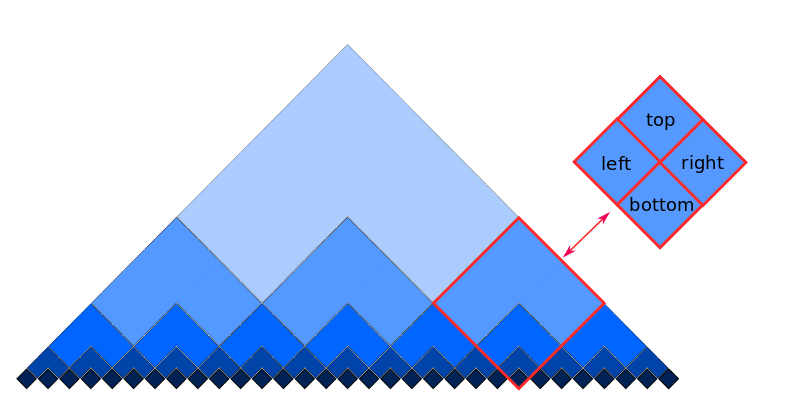
\includegraphics[width=0.9\textwidth]{Susanina/pics/layers.png}
    \caption{Деление матриц на V-образные слои}
    \label{fig2}
 \end{center}
\vspace{-8mm}
\end{figure}

Пример работы алгоритма показан на рис.~\ref{modvis}. Нижний слой, состоящий из подматриц размера 1, вычисляется заранее, а заполнение матрицы начинается со второго слоя. (Здесь и далее, под слоем матриц будем понимать некоторое множество её подматриц разбора.) Более того, на рис. 4 на каждом шаге изображены операции, которые могут быть выполненные независимо, что позволяет значительно упростить разработку параллельной версии алгоритма.

\begin{figure}[h]
\vspace{3mm}
 \begin{center}
    \centering
    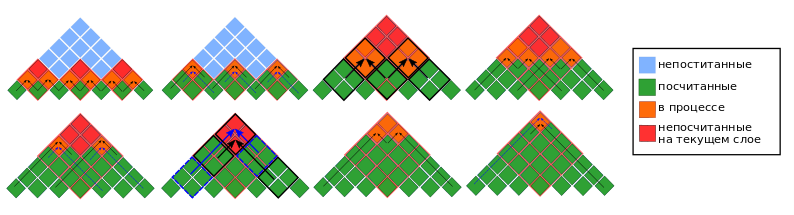
\includegraphics[width=0.9\textwidth]{Susanina/pics/modivis2.png}
    \caption{Деление матриц на V-образные слои}
    \label{modvis}
 \end{center}
\vspace{-8mm}
\end{figure}

Функция \textit{main()} (см. алгоритм 2) заполняет диагональ:  $(T_{l, l+1})$, затем делит матрицу на слои и вычисляет их с помощью процедуры \textit{completeVLayer()}.

Дополнительные функции \textit{left(subm)}, \textit{right(subm)}, \textit{top(subm)}, \textit{bottom(subm)}, \textit{rightgrounded(subm)} and \textit{leftgrounded(subm)} возвращают подматрицы матрицы $\textit{subm} = (l, m, l', m')$ аналогично алгоритму~\ref{algo:valiant}.

Процедура \textit{completeVLayer(M)} на вход принимает слой (массив подматриц)  $M$ и для каждой \textit{subm = (l, m, l', m') $\in M$} заполняет \textit{left(subm), right(subm), top(subm)}.
Предполагается, что \textit{bottom(subm)} и $T_{i, j}$ для всех $i$, $j$, таких что $l \leq i < j < m$, $  l' \leq i < j < m'$ уже корректно вычислены и
$P_{i, j} =  \{ (B, C) | \exists k, (m \le k < l'), a_{i + 1} \dots a_{k} \in L_G(B), a_{k + 1} \dots a_{j} \in L_G(C)\} $ для всех $i$, $j$, таких что $l \leq i < m$, $l' \leq j < m'$.


\begin{algorithm}[!ht]
\hspace*{\algorithmicindent} \textbf{Вход:} {$G = (\Sigma, N, R, S), w = a_{1} \dots a_{n}, n + 1 = 2^p, a_{i} \in \Sigma$}
\begin{algorithmic}[1]
\Procedure{main}{}
 \For {$l \in \{1, \ldots, n \}$}{$T_{l, l + 1} = \{A \mid A \rightarrow a_{l + 1} \in R\}$}
 \EndFor
 \For{$1 \le i < p - 1 $}
   \State{\textit{layer = constructLayer($i$)}}
   \State{\textit{completeVLayer(layer)}}
 \EndFor
\EndProcedure

\Procedure{constructLayer}{i}
 \State{$\{(k2^i, (k+1)2^i, (k + 1)2^i, (k+2)2^i) \mid 0 \le k < 2^{p - i} - 1\}$}
\EndProcedure

\Procedure{completeLayer}{M}
\If {$\forall (l, m, l', m') \in M \quad (m - l = 1)$}{\For{$ (l, m, l', m') \in M$}{$T_{l, l'} = f(P_{l, l'})$}\EndFor}
\Else
\State{\textit{completeLayer($\{\textit{bottom(subm)}\, |\,\textit{subm} \in M \})$}}
\State{\textit{completeVLayer(M)}}
\EndIf
\EndProcedure

\Procedure{completeVLayer}{M}
 \State{$m_1 = \{\textit{left(sm)}, \textit{leftgrounded(sm)}, \textit{bottom(sm)} \mid \textit{sm} \in M \}$}
 \State{$\textit{mltTsk}_1 = m_1 \cup  \{\textit{right(s)}, \textit{bottom(s)}, \textit{rightgrounded(s)} \mid \textit{s} \in M\}$}
 \State{\textit{mltTsk$_2$} = $\{\textit{top(sm)}, \textit{leftgrounded(sm)}, \textit{right(sm)} \mid \textit{sm} \in M\}$}
 \State{\textit{mltTsk$_3$} = $\{\textit{top(sm)}, \textit{left(sm)}, \textit{rightgrounded(sm)} \mid \textit{sm} \in M\}$}
 \State{\textit{performMultiplications(mltTsk$_1$)}}
 \State{\textit{completeLayer($\{\textit{left(sm)} \mid sm \in M \} \cup \{\textit{right(sm)} \mid \textit{sm} \in M \}$)}}
 \State{\textit{performMultiplications(mltTsk$_2$)}}
 \State{\textit{performMultiplications(mltTsk$_3$)}}
 \State{\textit{completeLayer($\{top(sm) \mid sm \in M \}$)}}
\EndProcedure

\Procedure{performMultiplication}{tasks}
 \For{$ (m, m1, m2) \in \textit{tasks}$}{$P_{m} = P_{m} \cup (T_{m1} \times T_{m2})$}
 \EndFor
\EndProcedure
\end{algorithmic}

\caption{Алгоритм Явейн}
\label{algo:modified}
\end{algorithm}

Процедура \textit{completeLayer(M)} также принимает на вход массив матриц $M$, но заполняет $T_{i, j}$ для всех $(i, j) \in subm$.
Ограничение на $T_{i, j}$  and $P_{i, j}$ такие же, как в предыдущем случае, кроме условия на \textit{bottom(subm)}.

Другими словами, \textit{completeVLayer(M)} отвечает за заполнение слоя \textit{M}, а \textit{completeLayer($M_{2}$)} --- вспомагательная функция для вычисления для вычисления меньших матриц внутри слоя \textit{M}.

Теперь обратим внимание на процедуру \textit{performMultiplication(tasks)}, где \textit{tasks} --- массив троек подматриц, реализующий основной шаг алгоритма: перемножение матриц.
Здесь $|tasks| \ge 1$ и каждый $task \in tasks$ может быть выполнен параллельно, в отличие от алгоритма Валианта.

\subsection{Применение в биоинформатике и задача поиска подстрок}

Вторичная структура (определенный способ укладки биологической цепочки в сложную, упорядоченную структуру) генетических последовательностей, например, РНК, тесно связана с биологическими функциями организма, поэтому анализ таких последовательностей играет существеную роль в задачах распознавания и классификации.

Характерные черты вторичной структуры могут быть описаны с помощью КС-грамматики и, следовательно, часть подходов для анализа генетических последовательностей основаны на синтаксическом анализе. Главным недостатком таких подходов являются существенные проблемы с производительностью~\cite{durbin1996biological}, которые можно решить с помощью алгоритма Валианта.

Однако часто задачей является нахождение не одной, а всех подпоследовательностей, обладающих данными чертами. Для этой задачи алгоритм Валианта плохо применим,  так как его трудно остановить на определенном этапе заполнения матрицы разбора и это потребует много лишних перемножений матриц.
Предполагается, что алгоритм Явейн должен решить эту проблему, но сначала надо показать, что он не утратил преимущества исходного алгоритма.

\section{Доказательство корректности и оценка сложности алгоритма Явейн}

В данном разделе мы приведем доказательство корректности алгоритма Явейн и дадим оценку его вычислительной сложности.

\begin{lemma}
Пусть процедура \textit{completeLayer(M')} с выполненными следующими ограничениями:
\begin{enumerate}
  \item $T_{i, j} = \{ A |  a_{i + 1} \dots a_{j} \in L_G(A)\}$ для всех $i$ и $j$, таких что $l1 \leq i < j < m1$ и $l2 \leq i < j < m2$;
  \item $P_{i, j} =  \{ (B, C) |\exists k, (m1 \le k < l2): a_{i + 1} \dots a_{k} \in L_G(B), a_{k + 1} \dots a_{j} \in L_G(C)\}$ для всех $l1 \leq i < m1$ и $l2 \leq j < m2$.
\end{enumerate}
возвращает для любого слоя $M'$ корректно заполненные $T_{i, j}$ для всех $l1 \leq i \le m1$ и $l2 \leq j \le m2$ при этом $(l1, m1, l2, m2) \in M'$
и пусть для слоя $M$ выполняется, что:
\begin{enumerate}
  \item $T_{i, j} = \{ A |  a_{i + 1} \dots a_{j} \in L_G(A)\}$ для всех $i$ и $j$, таких что $l \leq i < j < m$ и $l' \leq i < j < m'$ и для $(i, j) \in bottom(M)$;
  \item $P_{i, j} =  \{ (B, C) |\exists k, (m \le k < l'): a_{i + 1} \dots a_{k} \in L_G(B), a_{k + 1} \dots a_{j} \in L_G(C)\}$ для всех $l \leq i < m$ и $l' \leq j < m'$.
\end{enumerate}

Тогда процедура \textit{completeVLayer(M)} возвращает корректно заполненные $T_{i, j}$ при этом $l \leq i \le m$ и $l' \leq j \le m'$ для всех $(l, m, l', m') \in M$.
\end{lemma}

\begin{proof}

\textit{performMultiplications(mltTsk$_1$)} добавит к каждому P$_{i,j}$ все пары
$(B, C)$, такие что $\exists k$, $(\frac{l+m}{2} \le k < l')$, $a_{i + 1} \dots a_{k} \in L_{G}(B)$, $a_{k + 1} \dots a_{j} \in L_{G}(C)$ для всех $(i, j)$ $\in leftsublayer(M)$
и
$(B, C)$, такие что $\exists k$, $(m \le k < \frac{l'+m'}{2})$, $a_{i + 1} \dots a_{k} \in L_{G}(B)$, $a_{k + 1} \dots a_{j} \in L_{G}(C)$ для всех $(i, j)$ $\in rightsublayer(M)$.
Теперь, так как все ограничения соблюдены, можно вызвать \textit{completeLayer(leftsublayer(M) $\cup$ rightsublayer(M))} и она вернет корректно заполненные \textit{leftsublayer(M) $\cup$ rightsublayer(M)}.

Далее функция \textit{performMultiplications}, вызванная от аргументов
\textit{mltTsk$_2$} и \textit{mltTsk$_3$}, к каждому P$_{i,j}$ добавит все пары
$(B, C)$, такие что $\exists k$, $(\frac{l+m}{2} \le k < m)$, $a_{i + 1} \dots a_{k} \in L_{G}(B)$, $a_{k + 1} \dots a_{j} \in L_{G}(C)$
и все пары
$(B, C)$, такие что $\exists k$, $(l' \le k < \frac{l'+m'}{2})$, $a_{i + 1} \dots a_{k} \in L_{G}(B)$, $a_{k + 1} \dots a_{j} \in L_{G}(C)$
для всех $(i, j)$ $\in topsublayer(M)$.
Так как $m = l'$ (из построения слоя), ограничения на элементы $P$ выполнены.
И процедура \textit{completeLayer(topsublayer(M))} может быть вызвана и она вернет корректно заполненные \textit{topsublayer(M)}.

Теперь $\forall (i, j) \in M$ $T_{i, j}$ заполены корректно.

\end{proof}

\begin{theorem}
Пусть $M$ --- слой, и для всех $(l, m, l', m') \in M$ справедливо:
\begin{enumerate}
  \item $T_{i, j} = \{ A |  a_{i + 1} \dots a_{j} \in L_G(A)\}$ для всех $i$ и $j$, таких что $l \leq i < j < m$ и $l' \leq i < j < m'$;
  \item $P_{i, j} =  \{ (B, C) |\exists k, (m \le k < l'): a_{i + 1} \dots a_{k} \in L_G(B), a_{k + 1} \dots a_{j} \in L_G(C)\}$ для всех $l \leq i < m$ и $l' \leq j < m'$.
\end{enumerate}

Тогда процедура \textit{completeLayer(M)} возвращает корректно заполненные $T_{i, j}$ для всех $l \leq i \le m$ и $l' \leq j \le m'$ при этом $(l, m, l', m') \in M$.
\end{theorem}


\begin{proof}(Индукция по $m - l$.)

Будем рассматривать одну матрицу $(l, m, l', m')$, так как для остальных матриц процесс заполнения производится аналогично.

\underline{База индукции:} $m - l = 1$. Необходимо вычислить всего один элемент и $P_{l, l'} =  \{ (B, C) |  a_{l + 1} \dots a_{l'} \in L(B)L(C)\}$. Алгоритм вычисляет $f(P_{l, l'}) = \{ A |  a_{l + 1} \dots a_{l'} \in L(A)\}$ и $T_{l, l'}$ теперь заполнена корректно.

\underline{Индукционный переход:} Предположим, что $(l_1, m_1, l_2, m_2)$ корректно заполняются для всех $m_2 - l_2 = m_1 - l_1 < m - l$.

Рассмотрим вызов \textit{completeLayer(M)}, где $m - l > 1$.

Все ограничения на вызов \textit{completeLayer(bottomsublayer(M))} выполнены и $T_{i, j}$ будут корректно заполнены для всех $(i, j) \in bottomsublayer(M)$. Стоит отдельно упомянуть, что условия теоремы позволяют корректно заполнить самый нижний элемент $T_{m, l'}$ (аналогично тому, как это сделано в базе индукции).
Слой \textit{bottomsublayer(M)} теперь заполнен и можно вызвать процедуру \textit{completeVLayer(M)}.

Все $T_{i,j}$ уже заполнены для всех $i$ и $j$, таких что $l \leq i < j < m$ и $l' \leq i < j < m'$ из условий теоремы, следовательно теперь мы можем применить лемму 1. Это значит, что $T_{i, j}$ $\forall (i, j) \in M$ будут заполнены корректно.
\end{proof}

\begin{theorem}
Алгоритм Явейн (см. алгоритм ~\ref{algo:modified}) корректно заполняет $T_{i, j}$ для всех i и j, и входная строка $a = a_{1}a_{2} \dots a_{n} \in L_{G}(S)$ тогда и только тогда, когда $S \in T_{0, n}$.
\end{theorem}

\begin{proof}

Докажем по индукции, что все слои матрицы разбора $T$ вычисляются корректно.

\underline{База индукции:} Слой размера 1 × 1 корректно заполняется в строках 2-3 листинга 2.

\underline{Индукционный переход:} Предположим, что все слои размера $\le 2^{p - 2} \times 2^{p - 2}$ вычислены корректно.

Обозначим слой размера $2^{p - 1} \times 2^{p - 1}$ как $M$. Будем рассматривать одну матрицу слоя \textit{subm = (l, m, l', m')}, так как для остальных подматриц их заполнение будет проходить аналогично.

Рассмотрим вызов процедуры \textit{completeVLayer(M)} call.
$T_{i,j}$ для всех $i$ и $j$ таких, что $l \leq i < j < m$ и $l' \leq i < j < m'$, уже корректно заполнены, так как эти элементы лежат в слоях, которые уже вычислены по индукционному предположению.

Все условия леммы 1 и теоремы 1 выплнены. Следовательно, \textit{completeVLayer(M)} возвращает корректно заполненные $T_{i, j}$ для всех $(i, j)$ $\in M$ для каждого слоя $M$ матрицы разбора $T$ и строки 4-6 листинга~\ref{algo:modified} возвращают все $T_{i, j} =  \{ A | A \in N, a_{i + 1} \dots a_{j} \in L_{G}(A)\}$.

\end{proof}

\begin{lemma}
Пусть \textit{calls$_{i}$} --- это количество вызовов процедуры \textit{completeVLayer(M)}, где для всех $(l, m, l', m') \in M$ выполняется $m - l = 2^{p - i}$. Тогда истинны следующие утверждения:
\begin{itemize}
 \item для всех $i \in \{ 1, .., p - 1\}$  $\sum_{n=1}^{calls_i}{|M|} = 2^{2i - 1} - 2^{i - 1}$;
 \item для всех $ i \in \{ 1, .., p - 1\}$ матрицы размера $2^{p - i} \times 2^{p - i}$ перемножаются ровно $2^{2i - 1} - 2^{i}$ раз.
\end{itemize}
\end{lemma}

\begin{proof}

Сначала докажем первое утверждение индукцией по $i$.

\underline{База индукции:} i = 1. \textit{calls$_{1}$} и $|M| = 1$. So, $2^{2i - 1} - 2^{i - 1} = 2^1 - 2^0 = 1$.

\underline{Индукционный переход:} предположим, что $\sum_{n=1}^{calls_i}{|M|} = 2^{2i - 1} - 2^{i - 1}$ для всех $i \in \{ 1, .., j\}$.

Пусть $i = j + 1$.

Заметим, что функция $\textit{costructLayer(i)}$ возвращает $2^{p - i} - 1$ матриц размера $2^i$, то есть в вызове процедуры \textit{completeVLayer(costructLayer(k - i))}  \textit{costructLayer(k - i)} вернет $2^i - 1$ матриц размера $2^{p - i}$.
Также процедура \textit{completeVLayer(M)} будет вызвано 3 раза для левых, правых и верхних подматриц матриц размера $2^{p - (i - 1)}$. Кроме того, \textit{completeVLayer(M)} вызывается 4 раза для нижних, левых, правых и верхних подматриц матриц размера $2^{p - (i - 2)}$, за исключением левых, правых и верхних подматриц матриц размера $2^{i - 2} - 1$, которые к этому моменту уже были посчитаны.

Таким образом, $\sum_{n=1}^{calls_i}{|M|} = 2^{i} - 1 + 3 \times (2^{2(i - 1) - 1} - 2^{(i - 1) - 1}) + 4 \times (2^{2(i - 2) - 1} - 2^{(i - 2) - 1}) - (2^{i - 2} - 1) = 2^{2i - 1} - 2^{i - 1}$.

Теперь мы знаем, что $\sum_{n=1}^{calls_{i-1}}{|M|} = 2^{2(i - 1) - 1} - 2^{(i - 1) - 1}$, и можем доказать второе утверждение. Посчитаем количество перемножений матриц размера $2^{p - i} \times 2^{p - i}$.
Процедура \textit{performMultiplications} вызывается 3 раза, $|mltTsk_1| = 2 \times 2^{2(i - 1) - 1} - 2^{(i - 1) - 1}$ и $|mltTsk_2|$ = $|mltTsk_3| = 2^{2(i - 1) - 1} - 2^{(i - 1) - 1}$. То есть, количество перемножений подматриц размера $2^{p - i} \times 2^{p - i}$ равно $ 4 \times (2^{2(i - 1) - 1} - 2^{(i - 1) - 1}) = 2^{2i - 1} - 2^{i}$.
\end{proof}

\begin{theorem}
Пусть $|G|$ --- длина описания грамматики $G$, n --- длина входной строки. Тогда алгоритм из листинга~\ref{algo:modified} заполняет матрицу разбора \textit{T} за $\mathcal{O}(|G|BMM(n)\log{n})$, где $BMM(n)$ --- количество операций, необходимое для перемножения двух булевых матриц размера $n \times n$.
\end{theorem}

\begin{proof}
Так как в лемме 2 было показано, что количество перемножений матриц не изменилось по сравнению с исходной версией алгоритма Валианта, то доказательство будет идентично доказательству теоремы 1~\cite{Okhotin:2014:PMM:2565359.2565379}.
\end{proof}

Таким образом, мы доказали корректность алгоритма Явейн, а также показали, что его сложность осталась такой же, как и сложность исходного алгоритма Валианта.


\section{Анализ эффективности применения к задаче поиска подстрок алгоритмов Валианта и Явейн}

В данном разделе мы продемонстрируем, как алгоритм Явейн может быть применен к задаче поиска подстрок.
Пусть мы хотим для входной строки размера $n = 2^p$ найти все подстроки размера $s$, которые принадлежат языку, заданному грамматикой $G$.
Тогда мы должны посчитать слои подматриц, размер которых не превышает $2^{r}$, где $2^{r - 2} < s \le 2^{r - 1}$.

Пусть $r = p - (m - 2)$ и, следовательно, $(m - 2) = p - r$.
Для всех  $m \le i \le p$ перемножение матриц размера $2^{p - i}$ выполняется ровно $2^{2i - 1} - 2^{i}$ раз и каждое из них включает перемножение $\mathcal{O}(|G|)$ булевых подматриц.

\begin{equation*}
\begin{array}{c}
C \sum\limits_{i=m}^p 2^{2i - 1} \cdot 2^{\omega(p - i)} \cdot f(2^{p - i}) = \\
C \cdot 2^{\omega l'}\sum\limits_{i=2}^{r} 2^{(2 - \omega)i} \cdot 2^{2(p - r) - 1} \cdot f(2^{r - i}) \le \\
C \cdot 2^{\omega r} f(2^{r}) \cdot 2^{2(p - r) - 1} \sum\limits_{i=2}^{r} 2^{(2 - \omega)i} = \\
BMM(2^{r}) \cdot 2^{2(p - r) - 1} \sum\limits_{i=2}^{r} 2^{(2 - \omega)i}
\end{array}
\end{equation*}

Временная сложность алгоритма для поиска всех подстрок длины $s$ равна $\mathcal{O}(|G|2^{2(p - r) - 1}BMM(2^{r})(r - 1))$, где появившийся дополнительный множитель обозначает количество матриц в последнем вычисленном слое, но он, во-первых, мал относительно общей работы алгоритма, во-вторых, не существенен, так как эти матрицы могут быть обработаны параллельно.

\begin{figure}[h]
\vspace{3mm}
 \begin{center}
 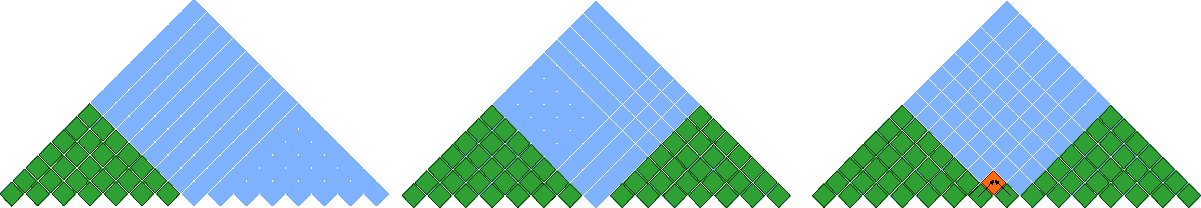
\includegraphics[width=0.9\textwidth]{Susanina/pics/valsubstring.pdf}
    \caption{Количество элементов, вычисляемых в алгоритме Валианта (2  треугольные подматрицы размера $\frac{n}{2}$), выделенные зеленым цветом.}
    \label{fig5}
 \end{center}
\vspace{-8mm}
\end{figure}

Алгоритм Валианта, в отличие от модификации, не может так легко быть применен к данной задаче. В нем необходимо будет полностью вычислить, как минимум, две треугольные подматрицы размера $\frac{n}{2}$, как показано на рис.~\ref{fig5}.
Это значит, что минимальная сложность, улучшить которую без дополнительных модификаций не удастся, будет составлять $\mathcal{O}(|G|BMM(2^{p - 1})(p - 2))$.

Таким образом, в данном разделе мы показади, что алгоритм Явейн может быть эффективно применен для строк размера $s \ll n$.



\section{Реализация алгоритмов Валианта и Явейн}

В рамках данной работы мы реализовали алгоритм Явейн несколькими способами. Мы хотели исследовать, как повлияют на производительность те или иные особенности каждой реализации. Также был реализован исходный алгоритм Валианта для сравнения и проверки эффективности модифицированного алгоритма.

\subsection{Последовательная версия}

Первая реализизация основана на использовании уже существующих библиотек.
Языком программирования был выбран С++. Для перемножения матриц была использована библиотека для работы с плотними матрицами --- M4RI~\cite{M4RI}.
Данная библиотека была выбрана, так как там реализован один их наиболее эффективных способов перемножения булевых матриц --- метод четырех русских~\cite{albrechtefficient, arlazarov1970economical}.

\subsection{Параллельная версия}

Далее мы решили остановиться на использовании параллельных техник, а именно GPGPU (General-purpose computing on graphics processing units). Была создана простая реализация перемножения подматриц на языке программирования CUDA С~\cite{nvidia2011nvidia}. Это расширение языка C, позволяющее создавать эффективные программы за счет использования возможностей графических процессоров.  Использование параллельных вычислений происходит сразу на трех уровнях: само перемножение матриц (каждый элемент результирующий матрицы обрабатывается независимо), перемножение булевых матриц для каждой пары нетерминалов, которым соответствует хотя бы одно правило, и перемножение подматриц слоя для алгоритма Явейн.


\section{Эксперименты}

В данной секции мы приводим результаты экспериментов, целью которых было исследование производительности и практической применимости алгоритма Явейн.

Эксперименты проводились на рабочей станции со следующими характеристиками:
\begin{itemize}
    \item операционная система: Linux Mint 19.1;
    \item ЦПУ: Intel i5-8250U, 1600-3400 Mhz, 4 Core(s), 8 Logical Processor(s);
    \item объем оперативной памяти: 8.0 GB;
    \item графический процессор: NVIDIA GeForce GTX-1050.
\end{itemize}

Основной целью поставленных экспериментов было исследование возможностей алгоритма Явейн.
Для этого были поставлены следующие вопросы.

Q1. Сравнение алгоритмов Валианта и Явейн.

Q2. Эффективность применения алгоритма Явейн к задаче поиска подстрок.

Для ответа на вопрос Q1 был проведен сравнительный анализ как последовательной, так и параллельной версий реализации алгоритмов Валианта и Явейн.

При исследовании алгоритмы были протестированы на двух грамматиках. Сначала была выбрана грамматика Дика для двух типов скобок ($D2$) ~\cite{hopcroft1969formal}, потому что грамматики для описания правильных скобочных последовательностей применяются при анализе строк в биоинформатике. Она представлена на листинге~\ref{dyck}.

\begin{listing}
\caption{Грамматика $D2$}

\quad\quad\quad\quad\quad\quad\quad\quad\quad\quad\quad\quad s : s s  |  (s) |  [s]  |  $\epsilon$

\label{dyck}
\end{listing}

Грамматика $D2$ переводится в нормальную форму Хомского и подается на вход алгоритму со специально сгенерированными строками различной длины (127-8191 символов). Строки составлены следующим образом: заранее создается подстрока, принадлежащая языку Дика, далее в полную строку вставляется максимально возможное количество созданных подстрок, которые можно разделить “перегородками” (терминалами, из-за которых все остальные строки, кроме вставленных, будут невыводимыми в грамматике $D2$). Строки были созданы таким образом, чтобы проверять корректность предложенного алгоритма.

Второй грамматикой для тестирования производительности алгоритмов была выбрала грамматика, применяющаяся в некоторых работах по биоинформатике ($BIO$)~\cite{bioinformatics19}. Она представлена на листинге~\ref{bio}. Грамматика $BIO$ также, как и в предыдущем случае, переводится в нормальную форму Хомского. Строки для данного эксперимента были сгенерированны случайным образом.

\begin{listing}[h]
\caption{Грамматика $BIO$}
\begin{pyglist}[]
            s1: stem<s0>
            any_str : any_smb*[2..10]
            s0: any_str | any_str stem<s0> s0
            any_smb: A | T | C | G
            stem1<s>: A s T | G s C | T s A | C s G
            stem2<s>: stem1<stem1<s>>
            stem<s>:
                  A stem<s> T
                | T stem<s> A
                | C stem<s> G
                | G stem<s> C
                | stem1<stem2<s>>
\end{pyglist}
\label{bio}
\end{listing}


Для ответа на вопрос Q2 в алгоритме Явейн была изменена функция $main()$: теперь она принимает дополнительный аргумент s --- длину максимальной искомой подстроки и вычисляет только те слои, которые содержат в себе нужные подстроки, как было показано в разделе 4. Далее версию алгоритма Явейн с измененной функцией $main()$ будем называть адаптированнной к задаче поиска подстрок. Тестирование проводилось на грамматиках $D2$ и $BIO$, строки были сгенерированы также, как и в предыдущем случае.


\subsection{Сранительный анализ}

Результаты сравнительного анализа реализаций алгоритма Валианта и Явейн представлены в таблице~\ref{tbl1} и на рис.~\ref{expPlots}.
При этом $N$ –-- это длина сгенерированной строки, valCPU --- последовательная реализация алгоритма Валианта, yavCPU --- последовательная реализация алгоритма Явейн, valGPU --- параллельная реализация алгоритма Валианта и yavGPU --- параллельная версия алгоритма Явейн.
Время работы алгоритмов представленно в таблице~\ref{tbl1}  в миллисекундах.

\begin{table}[h]
\caption{Результаты сравнительного анализа (время в мс)}
\label{tbl1}
\centering
\resizebox{\columnwidth}{!}{%
\begin{tabular}{|| c||c|c|c|c || c|c|c|c ||}
\hline
\multirow{2}{1em}{N} & \multicolumn{4}{c||}{Грамматика $D2$} & \multicolumn{4}{c||}{Грамматика $BIO$} \\
& valCPU & yavCPU & valGPU & yavGPU & valCPU & yavCPU & valGPU & yavGPU \\
\hline
127 & 78 & 76 & 195 & 105 & 1345 & 1339 & 193 & 106 \\
255 & 289 & 292 & 523 & 130 & 5408 & 5488 & 525 & 140 \\
511 & 1212 & 1177 & 1909 & 250 & 21969 & 22347 & 1994 & 256 \\
1023 & 4858 & 4779 & 7878 & 540 & 88698 & 90318 & 7890 & 598 \\
2047 & 19613 & 19379 & 33508 & 1500 & 363324 & 374204 & 34010 & 1701 \\
4095 & 78361 & 78279 & 140473 & 4453 & 1467675 & 1480594 & 141104 & 5472 \\
8191 & 315677 & 315088 & - & 13650 & - & - & - & 18039 \\
\hline
\end{tabular}
}
\end{table}

\begin{figure}[h]
\centering
\begin{minipage}[b]{.5\linewidth}
    \begin{tikzpicture}[scale=.5]
    \begin{axis}[
    legend cell align=left,
    legend pos = north west,
    xlabel = {Длина входной строки},
    ylabel = {Время, с},
    %ymode=log
    ]
    \addplot [color=blue, mark=triangle*] coordinates {
        (127, 0.078) (255, 0.289) (511,1.212) (1023,4.858) (2047,19.613) (4095,78.361)
    };
    \addplot [color=red, mark=*] coordinates {
        (127, 0.076) (255, 0.292) (511,1.177) (1023,4.779) (2047,19.379) (4095,78.279)
    };
    \legend{
        valCPU,
        yavCPU
    };
    \end{axis}%\caption
    \end{tikzpicture}
    \label{fig:GSSedges}
		\subcaption{\scriptsize Последовательная реализация}
	\end{minipage}
\begin{minipage}[b]{.45\linewidth}
\begin{tikzpicture}[scale=.5]linewidth
\begin{axis}[
legend cell align=left,
legend pos = north west,
xlabel = {Длина входной строки},
ylabel = {Время, с},
%ymode=log
]
\addplot [color=blue, mark=triangle*] coordinates {
(127, 0.195) (255, 0.523) (511,1.995) (1023,7.888) (2047,34.008) (4095,141.173)
};
\addplot [color=red, mark=*] coordinates {
(127, 0.105) (255, 0.140) (511,0.256) (1023,0.590) (2047,1.7) (4095,5.453)
};
\legend{
valGPU,
yavGPU
};
\end{axis}
\end{tikzpicture}
\subcaption{\scriptsize Параллельная реализация}
\label{fig:Time}
\end{minipage}
\caption{Результаты экспериментов с грамматикой $D2$.}
\label{expPlots}
\end{figure}


Результаты сравнительного анализа для последовательной версии показывают, что алгоритмы работают практически одинаково. Однако видно, как на последовательную реализацию влияет константа $|G|$ --- длина описания грамматики $G$. В нашем случае, для грамматики $D2$ количество правил при переводе в нормальную форму Хомского составляет 7, а для $BIO$ ---  106. Это означает, что скорость работы алгоритмов прямо пропорциональна количеству правил грамматики.

Параллельная версия алгоритма Валианта оказалась медленнее на грамматике $D2$. Можно предположить, что это связано с большим количеством перемножений матриц небольшого размера и невозможностью их параллельной обработки. Но на больших грамматиках ($BIO$) она демонстрирует значительное улучшение производительности по сравнению с последовательной версией за счет использования параллелизма на уровне правил грамматики (то есть независимого перемножения матриц для каждой пары нетерминалов).

Лучшее время работы показывает параллельная версия алгоритма Явейн. Это связано с тем, что параллелизм используется сразу на трех уровнях, как было замечено в предыдущем разделе.

\subsection{Применимость к задаче поиска подстрок}

Результаты работы адаптированного к задаче поиска подстрок алгоритма Явейн представлены в таблице~\ref{tbl3}. Здесь N --– это длина сгенерированной строки, s --- длина искомой подстроки, adpCPU --- время работы последовательной реализации адаптированного алгоритма Явейн, adpGPU --- время работы параллельной реализации адаптированнного алгоритма Явейн.
Время работы на таблице~\ref{tbl3} представлено в миллисекундах.

\begin{table}[h]

\begin{center}
\caption{Результаты работы алгоритма Явейн для задачи поиска подстрок (время в мс)}
\label{tbl3}
    \begin{tabular}{ ||c||c||c|c|| }
    \hline
    s & N & adpCPU &  adpGPU \\
    \hline
    \multirow{4}{2em}{250} & 1023 & 2996 & 242 \\
    & 2047 & 6647 & 255\\
    & 4095 & 13825 & 320\\
    & 8191 & 28904 & 456\\
    \hline
    \multirow{3}{2em}{510} & 2047 & 12178 & 583\\
    & 4095 & 26576 & 653\\
    & 8191 & 56703 & 884\\
    \hline
    \multirow{2}{2em}{1020} & 4095 & 48314 & 1590 \\
    & 8191 & 108382 & 1953\\
    \hline
    2040 & 4095 & 197324 & 5100\\
    \hline
    \end{tabular}
\end{center}

\end{table}


Результаты второго эксперимента показывают, что адаптированная версия алгоритма Явейн может быть эффективно применена к задаче поиска подстрок: она корректно находит все выводимые подстроки в строке и работает существенно быстрее алгоритма Валианта (см. таблицу~\ref{tbl1}), который будет совершать большое количество лишних вычислений из-за сложности его преждевременной остановки.

Таким образом, проведенные эксперименты показали практическую применимость алгоритма Явейн, возможность его существенного ускорения за счет использования параллельных вычислений и адаптации к задаче поиска подстрок.

\section{Заключение}
В данной работе были получены следующие результаты.

\begin{itemize}
	\item Доказана корректность алгоритма Явейн и дана оценка вычислительной сложности, которая составляет $\mathcal{O}(BMM(n)log(n))$.
	\item Проведен анализ, который показал, что алгоритм Явейн лучше применим к задаче поиска подстрок, чем алгоритм Валианта.
	\item Реализованы последовательная и параллельная версии алгоритмов. Исходный код доступен в репозитории: \url{https://github.com/SusaninaJulia/PBMM}.
	\item Проведено экспериментальное исследование алгоритма, показавшее эффективность алгоритма Явейн: последовательные версии алгоритмов Валианта и Явейн работают одинаково; параллельная версия алгоритма Явейн показывает значительный прирост производительности на строках большей длины; показана эффективность применения алгоритма Явейн к задаче поиска подстрок.
	\item Результаты работы приняты к публикации в журнале <<Труды ИСП РАН>>.
\end{itemize}

Кроме того, мы можем определить несколько направлений будущих исследований.
Например, оптимизация алгоритмов перемножения матриц за счет использования разделяемой памяти позволит повысить производительность алгоритмов.
Еще планируется расширить алгоритм Явейн для других классов грамматик, которые применяются в биоинформатике: конъюнктивных и булевых.
Также, открытым остается вопрос, можно ли как-либо изменить порядок перемножения подматриц, чтобы полностью избавить алгоритм от рекурсивных вызовов.

\begin{thebibliography}{10}
\def\selectlanguageifdefined#1{
\expandafter\ifx\csname date#1\endcsname\relax
\else\selectlanguage{#1}\fi}
\providecommand*{\href}[2]{{\small #2}}
\providecommand*{\url}[1]{{\small #1}}
\providecommand*{\BibUrl}[1]{\url{#1}}
\providecommand{\BibAnnote}[1]{}
\providecommand*{\BibEmph}[1]{#1}
\ProvideTextCommandDefault{\cyrdash}{\iflanguage{russian}{\hbox
  to.8em{--\hss--}}{\textemdash}}
\providecommand*{\BibDash}{\ifdim\lastskip>0pt\unskip\nobreak\hskip.2em plus
  0.1em\fi
\cyrdash\hskip.2em plus 0.1em\ignorespaces}
\renewcommand{\newblock}{\ignorespaces}

\bibitem{IDGrammar}
\selectlanguageifdefined{english}
\BibEmph{Alur~Rajeev, Madhusudan~P.}
  \href{http://dx.doi.org/10.1145/1007352.1007390}{Visibly Pushdown
  Languages}~// Proceedings of the Thirty-sixth Annual ACM Symposium on Theory
  of Computing. \BibDash
\newblock STOC '04. \BibDash
\newblock New York, NY, USA~: ACM, 2004. \BibDash
\newblock P.~202--211.

\bibitem{MatrixMult}
\selectlanguageifdefined{english}
\BibEmph{Azimov~Rustam, Grigorev~Semyon}. Graph Parsing by Matrix
  Multiplication~// Proceedings of the 1st ACM SIGMOD Joint International Workshop on Graph Data Management Experiences \& Systems (GRADES) and Network Data Analytics (NDA). \BibDash
\newblock GRADES-NDA '18 \BibDash
\newblock New York, NY, USA~: ACM, 2018.
\newblock P.~5:1--5:10.

\bibitem{ConjPath}
\selectlanguageifdefined{english}
\BibEmph{Azimov~Rustam, Grigorev~Semyon}. Path querying using conjunctive
  grammars~//
  \href{http://dx.doi.org/10.15514/ISPRAS-2018-30(2)-8}{\BibEmph{Proceedings of
  the Institute for System Programming of the RAS}}. \BibDash
\newblock 2018. \BibDash 01. \BibDash
\newblock Vol.~30. \BibDash
\newblock P.~149--166.

\bibitem{GraphDB}
\selectlanguageifdefined{english}
\BibEmph{Barceló~Baeza~Pablo}. Querying graph databases~//
  \href{http://dx.doi.org/10.1145/2463664.2465216}{\BibEmph{Proceedings of the
  ACM SIGACT-SIGMOD-SIGART Symposium on Principles of Database Systems}}.
  \BibDash
\newblock 2013. \BibDash 06.

\bibitem{Bradford}
\selectlanguageifdefined{english}
\BibEmph{Bradford~Phillip~G.} Efficient Exact Paths For Dyck and semi-Dyck
  Labeled Path Reachability~// \BibEmph{CoRR}. \BibDash
\newblock 2018. \BibDash
\newblock Vol. abs/1802.05239. \BibDash
\newblock 1802.05239.

\bibitem{Brent}
\selectlanguageifdefined{english}
\BibEmph{Brent~Richard, M.~GOLDSCHLAGER~LESLIE}. A PARALLEL ALGORITHM FOR
  CONTEXT-FREE PARSING. \BibDash
\newblock 1983. \BibDash 01.

\bibitem{social}
\selectlanguageifdefined{english}
\BibEmph{Chaudhary~Anoop, FAISAL~ABDUL}. Role of graph databases in social
  networks. \BibDash
\newblock 2016. \BibDash 06.

\bibitem{Lohrey}
\selectlanguageifdefined{english}
Circuits and Expressions over Finite Semirings~/ Moses~Ganardi, Danny~Hucke,
  Daniel~König, Markus~Lohrey~//
  \href{http://dx.doi.org/10.1145/3241375}{\BibEmph{ACM Transactions on
  Computation Theory}}. \BibDash
\newblock 2018. \BibDash 08. \BibDash
\newblock Vol.~10. \BibDash
\newblock P.~1--30.

\bibitem{RDF}
\selectlanguageifdefined{english}
Context-Free Path Queries on {RDF} Graphs~/ Xiaowang~Zhang, Zhiyong~Feng,
  Xin~Wang, Guozheng~Rao~// \BibEmph{CoRR}. \BibDash
\newblock 2015. \BibDash
\newblock Vol. abs/1506.00743. \BibDash
\newblock 1506.00743.

\bibitem{Dyck1}
\selectlanguageifdefined{english}
\BibEmph{Deleage~Jean-Luc, Pierre~Laurent}. The rational index of the Dyck
  language $D_1$~//
  \href{http://dx.doi.org/10.1016/0304-3975(86)90158-1}{\BibEmph{Theoretical
  Computer Science}}. \BibDash
\newblock 1986. \BibDash
\newblock Vol.~47. \BibDash
\newblock P.~335 -- 343.

\bibitem{Dymond}
\selectlanguageifdefined{english}
\BibEmph{Dymond~Patrick~W.} Input-driven languages are in log n depth~//
  \href{http://dx.doi.org/10.1016/0020-0190(88)90148-2}{\BibEmph{Information
  Processing Letters}}. \BibDash
\newblock 1988. \BibDash
\newblock Vol.~26, no.~5. \BibDash
\newblock P.~247 -- 250.

\bibitem{Earley}
\selectlanguageifdefined{english}
\BibEmph{Earley~Jay}. An Efficient Context-free Parsing Algorithm~//
  \href{http://dx.doi.org/10.1145/362007.362035}{\BibEmph{Commun. ACM}}.
  \BibDash
\newblock 1970. \BibDash Feb. \BibDash
\newblock Vol.~13, no.~2. \BibDash
\newblock P.~94--102.

\bibitem{PCompl}
\selectlanguageifdefined{english}
\BibEmph{Greenlaw~Raymond, Hoover~H.~James, Ruzzo~Walter~L.} Limits to Parallel
  Computation: P-completeness Theory. \BibDash
\newblock New York, NY, USA~: Oxford University Press, Inc., 1995. \BibDash
\newblock
  ISBN:~\href{http://isbndb.com/search-all.html?kw=0-19-508591-4}{0-19-508591-4}.

\bibitem{Ibarra}
\selectlanguageifdefined{english}
\BibEmph{H.~Ibarra~Oscar, Jiang~Tao, Ravikumar~Bala}. Some Subclasses of
  Context-Free Languages In NC1.~//
  \href{http://dx.doi.org/10.1016/0020-0190(88)90047-6}{\BibEmph{Inf. Process.
  Lett.}} \BibDash
\newblock 1988. \BibDash 10. \BibDash
\newblock Vol.~29. \BibDash
\newblock P.~111--117.

\bibitem{HellConj}
\selectlanguageifdefined{english}
\BibEmph{Hellings~Jelle}. Conjunctive Context-Free Path Queries~// ICDT.
  \BibDash
\newblock 2014.

\bibitem{HellingsCFPQ}
\selectlanguageifdefined{english}
\BibEmph{Hellings~Jelle}. Path Results for Context-free Grammar Queries on
  Graphs~// \BibEmph{CoRR}. \BibDash
\newblock 2015. \BibDash
\newblock Vol. abs/1502.02242. \BibDash
\newblock 1502.02242.

\bibitem{LLComp}
\selectlanguageifdefined{english}
\BibEmph{Holzer~Markus, Lange~Klaus~J{\"o}rn}. On the complexities of linear
  LL(1) and LR(1) grammars~// Fundamentals of Computation Theory~/ Ed.\ by\
  Zolt{\'a}n~{\'E}sik. \BibDash
\newblock Berlin, Heidelberg~: Springer Berlin Heidelberg, 1993. \BibDash
\newblock P.~299--308.

\bibitem{Kasami}
\selectlanguageifdefined{english}
\BibEmph{Kasami~Tadao}. AN EFFICIENT RECOGNITION AND SYNTAX ANALYSIS ALGORITHM
  FOR CONTEXT-FREE LANGUAGES. \BibDash
\newblock 1965. \BibDash 07. \BibDash
\newblock P.~40.

\bibitem{Kelemenova}
\selectlanguageifdefined{english}
\BibEmph{Kelemenová~Alica}. Complexity of normal form grammars~//
  \href{http://dx.doi.org/10.1016/0304-3975(83)90026-9}{\BibEmph{Theoretical
  Computer Science}}. \BibDash
\newblock 1983. \BibDash
\newblock Vol.~28, no.~3. \BibDash
\newblock P.~299 -- 314.

\bibitem{LReach}
\selectlanguageifdefined{english}
\BibEmph{Komarath~Balagopal, Sarma~Jayalal, Sunil~K.~S.} On the Complexity of
  L-reachability~// \BibEmph{CoRR}. \BibDash
\newblock 2017. \BibDash
\newblock Vol. abs/1701.03255. \BibDash
\newblock \href{http://arxiv.org/abs/1701.03255}{1701.03255}.

\bibitem{Reg2}
\selectlanguageifdefined{english}
\BibEmph{Koschmieder~Andr{\'e}, Leser~Ulf}.
  \href{http://dx.doi.org/10.1007/978-3-642-31235-9_12}{Regular Path Queries on
  Large Graphs}~// Proceedings of the 24th International Conference on
  Scientific and Statistical Database Management. \BibDash
\newblock SSDBM'12. \BibDash
\newblock Berlin, Heidelberg~: Springer-Verlag, 2012. \BibDash
\newblock P.~177--194.

\bibitem{Reg1}
\selectlanguageifdefined{english}
\BibEmph{Mendelzon~Alberto~O., Wood~Peter~T.} Finding Regular Simple Paths in
  Graph Databases~//
  \href{http://dx.doi.org/10.1137/S009753979122370X}{\BibEmph{SIAM J. Comput.}}
  \BibDash
\newblock 1995. \BibDash Dec. \BibDash
\newblock Vol.~24, no.~6. \BibDash
\newblock P.~1235--1258.

\bibitem{boolean}
\selectlanguageifdefined{english}
\BibEmph{Okhotin~Alexander}. Boolean grammars~//
  \href{http://dx.doi.org/10.1016/j.ic.2004.03.006}{\BibEmph{Information and
  Computation}}. \BibDash
\newblock 2004. \BibDash
\newblock Vol. 194, no.~1. \BibDash
\newblock P.~19 -- 48.

\bibitem{OkhotinParse}
\selectlanguageifdefined{english}
\BibEmph{Okhotin~Alexander}. Parsing by matrix multiplication generalized to
  Boolean grammars~//
  \href{http://dx.doi.org/10.1016/j.tcs.2013.09.011}{\BibEmph{Theoretical
  Computer Science}}. \BibDash
\newblock 2014. \BibDash
\newblock Vol. 516. \BibDash
\newblock P.~101 -- 120.

\bibitem{conjunctive}
\selectlanguageifdefined{english}
\BibEmph{Okhotin~Alexander}.
  \href{http://dx.doi.org/10.1007/978-3-319-98654-8_4}{A Tale of Conjunctive
  Grammars: 22nd International Conference, DLT 2018, Tokyo, Japan, September
  10-14, 2018, Proceedings}. \BibDash
\newblock 2018. \BibDash 01. \BibDash
\newblock P.~36--59. \BibDash
\newblock
  ISBN:~\href{http://isbndb.com/search-all.html?kw=978-3-319-98653-1}{978-3-319-98653-1}.

\bibitem{OkhotinIDPDA}
\selectlanguageifdefined{english}
\BibEmph{Okhotin~Alexander, Salomaa~Kai}. Complexity of Input-driven Pushdown
  Automata~// \href{http://dx.doi.org/10.1145/2636805.2636821}{\BibEmph{SIGACT
  News}}. \BibDash
\newblock 2014. \BibDash Jun. \BibDash
\newblock Vol.~45, no.~2. \BibDash
\newblock P.~47--67.

\bibitem{CFRat}
\selectlanguageifdefined{english}
\BibEmph{Pierre~Laurent}. Rational indexes of generators of the cone of
  context-free languages~//
  \href{http://dx.doi.org/10.1016/0304-3975(92)90269-L}{\BibEmph{Theoretical
  Computer Science}}. \BibDash
\newblock 1992. \BibDash
\newblock Vol.~95, no.~2. \BibDash
\newblock P.~279 -- 305.

\bibitem{GreibRat}
\selectlanguageifdefined{en}
\BibEmph{Pierre~Laurent, Farinone~Jean-Marc}. Context-free languages with
  rational index in $\Theta (n^\gamma )$ for algebraic numbers $\gamma $~//
  \BibEmph{RAIRO - Theoretical Informatics and Applications - Informatique
  Th\'eorique et Applications}. \BibDash
\newblock 1990. \BibDash
\newblock Vol.~24, no.~3. \BibDash
\newblock P.~275--322.

\bibitem{Bio}
\selectlanguageifdefined{english}
Quantifying variances in comparative RNA secondary structure prediction~/
  James~WJ~Anderson, {\'A}d{\'a}m~Nov{\'a}k, Zsuzsanna~S{\"u}k{\"o}sd et~al.~//
  \href{http://dx.doi.org/10.1186/1471-2105-14-149}{\BibEmph{BMC
  Bioinformatics}}. \BibDash
\newblock 2013. \BibDash May. \BibDash
\newblock Vol.~14, no.~1. \BibDash
\newblock P.~149.

\bibitem{Reps}
\selectlanguageifdefined{english}
\BibEmph{Reps~Thomas}. Program Analysis via Graph Reachability~// Proceedings
  of the 1997 International Symposium on Logic Programming. \BibDash
\newblock ILPS '97. \BibDash
\newblock Cambridge, MA, USA~: MIT Press, 1997. \BibDash
\newblock P.~5--19.

\bibitem{Reg3}
\selectlanguageifdefined{english}
\BibEmph{Reutter~Juan~L., Romero~Miguel, Vardi~Moshe~Y.} Regular Queries on
  Graph Databases~//
  \href{http://dx.doi.org/10.1007/s00224-016-9676-2}{\BibEmph{Theor. Comp.
  Sys.}} \BibDash
\newblock 2017. \BibDash Jul. \BibDash
\newblock Vol.~61, no.~1. \BibDash
\newblock P.~31--83.

\bibitem{QuadGreib}
\selectlanguageifdefined{english}
\BibEmph{Rosenkrantz~Daniel}. Matrix Equations and Normal Forms for
  Context-Free Grammars~//
  \href{http://dx.doi.org/10.1145/321406.321412}{\BibEmph{J. ACM}}. \BibDash
\newblock 1967. \BibDash 07. \BibDash
\newblock Vol.~14. \BibDash
\newblock P.~501--507.

\bibitem{LL}
\selectlanguageifdefined{english}
\BibEmph{Rosenkrantz~D.J., Stearns~R.E.} Properties of deterministic top-down
  grammars~//
  \href{http://dx.doi.org/10.1016/S0019-9958(70)90446-8}{\BibEmph{Information
  and Control}}. \BibDash
\newblock 1970. \BibDash
\newblock Vol.~17, no.~3. \BibDash
\newblock P.~226 -- 256.

\bibitem{Regularrealizability}
\selectlanguageifdefined{english}
\BibEmph{Rubtsov~Alexander~A., Vyalyi~Mikhail~N.} Regular realizability
  problems and context-free languages~// \BibEmph{CoRR}. \BibDash
\newblock 2015. \BibDash
\newblock Vol. abs/1503.00295. \BibDash
\newblock 1503.00295.

\bibitem{Ruzzo}
\selectlanguageifdefined{english}
\BibEmph{Ruzzo~Walter~L.} On uniform circuit complexity~//
  \href{http://dx.doi.org/10.1016/0022-0000(81)90038-6}{\BibEmph{Journal of
  Computer and System Sciences}}. \BibDash
\newblock 1981. \BibDash
\newblock Vol.~22, no.~3. \BibDash
\newblock P.~365 -- 383.

\bibitem{Rytter}
\selectlanguageifdefined{english}
\BibEmph{Rytter~Wojciech}. On the recognition of context-free languages~//
  Computation Theory~/ Ed.\ by\ Andrzej~Skowron. \BibDash
\newblock Berlin, Heidelberg~: Springer Berlin Heidelberg, 1985. \BibDash
\newblock P.~318--325.

\bibitem{Swernofsky2015OnTC}
\selectlanguageifdefined{english}
\BibEmph{Swernofsky~Joseph, Wehar~Michael}. On the Complexity of Intersecting
  Regular, Context-Free, and Tree Languages~// ICALP. \BibDash
\newblock 2015.

\bibitem{Tarjan}
\selectlanguageifdefined{english}
\BibEmph{{Tarjan}~R.} \href{http://dx.doi.org/10.1109/SWAT.1971.10}{Depth-first
  search and linear graph algorithms}~// 12th Annual Symposium on Switching and
  Automata Theory (swat 1971). \BibDash
\newblock 1971. \BibDash Oct. \BibDash
\newblock P.~114--121.

\bibitem{Valiant}
\selectlanguageifdefined{english}
\BibEmph{Valiant~Leslie~G.} General context-free recognition in less than cubic
  time~//
  \href{http://dx.doi.org/10.1016/S0022-0000(75)80046-8}{\BibEmph{Journal of
  Computer and System Sciences}}. \BibDash
\newblock 1975. \BibDash
\newblock Vol.~10, no.~2. \BibDash
\newblock P.~308 -- 315.

\bibitem{Yonger}
\selectlanguageifdefined{english}
\BibEmph{Younger~Daniel~H.} Recognition and parsing of context-free languages
  in time n3~//
  \href{http://dx.doi.org/10.1016/S0019-9958(67)80007-X}{\BibEmph{Information
  and Control}}. \BibDash
\newblock 1967. \BibDash
\newblock Vol.~10, no.~2. \BibDash
\newblock P.~189 -- 208.

\bibitem{DyckTrees}
\selectlanguageifdefined{english}
\BibEmph{Yuan~Hao, Eugster~Patrick}. An Efficient Algorithm for Solving the
  Dyck-CFL Reachability Problem on Trees~// Programming Languages and Systems~/
  Ed.\ by\ Giuseppe~Castagna. \BibDash
\newblock Berlin, Heidelberg~: Springer Berlin Heidelberg, 2009. \BibDash
\newblock P.~175--189.

\bibitem{Static}
\selectlanguageifdefined{english}
\BibEmph{Zhang~Qirun, Su~Zhendong}. Context-sensitive Data-dependence Analysis
  via Linear Conjunctive Language Reachability~//
  \href{http://dx.doi.org/10.1145/3093333.3009848}{\BibEmph{SIGPLAN Not.}}
  \BibDash
\newblock 2017. \BibDash Jan. \BibDash
\newblock Vol.~52, no.~1. \BibDash
\newblock P.~344--358.

\bibitem{Warcha2012UsingNG}
\selectlanguageifdefined{english}
\BibEmph{Łukasz Warchał}. Using Neo4j graph database in social network
  analysis. \BibDash
\newblock 2012.

\bibitem{UlmanCompilers}
\selectlanguageifdefined{russian}
Компиляторы: принципы, технологии и
  инструментарий~/ Д.~Ульман, Р.~Сети, М.~Лам,
  А.~Ахо. \BibDash
\newblock ЛитРес, 2018. \BibDash
\newblock
  ISBN:~\href{http://isbndb.com/search-all.html?kw=9785041399252}{9785041399252}.

\bibitem{Hopcroft}
\selectlanguageifdefined{russian}
\BibEmph{Хопкрофт~Д.~Мотвани~Р.~Ульман~Д.}
  Введение в теорию автоматов, языков и
  вычислений, 2-е издание. \BibDash
\newblock Издательский дом Вильямс. \BibDash
\newblock
  ISBN:~\href{http://isbndb.com/search-all.html?kw=9785845902610}{9785845902610}.

\end{thebibliography}

